\documentclass[a4paper]{article}
\usepackage[14pt]{extsizes} 
\usepackage[utf8]{inputenc}
\usepackage[english, russian]{babel}
\usepackage{amsmath}
\usepackage{amsfonts}
\usepackage{amssymb}
\usepackage{graphicx}
\usepackage{indentfirst}
\usepackage{mathtools}
\begin{document}
\begin{center}
\hfill \break
{\large МИНЕСТЕРСТВО НАУКИ ВЫСШЕГО ОБРАЗОВАНИЯ РОССИЙСКОЙ ФЕДЕРАЦИИ}\\
{\large Федеральное государственное бюджетное образовательное учереждение высшего образования}\\
\hfill \break
{\large \textbf{"КУБАНСКИЙ ГОСУДАРСТВЕННЫЙ УНИВЕРСИТЕТ"}} \\
\hfill \break
{\large \underline {Факультет}}\: Математики и Компьютерных Наук\\
{\large \underline {Направление }}\: Математики и Компьютерных Наук\\

\hfill \break
\hfill \break
\hfill \break
{\Large Лабораторная работа №3}\\
{\Large Вариант  №17}\\
\hfill \break \hfill \break
\hfill \break \hfill \break
Работу выполнил \underline{\hspace{7cm}} Батурин Н.Ю.\\
\hfill \break
Специальность \underline{02.03.01 математика и компьютерные науки } курс \underline{ 2}\\
\hfill \break
Специализация \underline{\hspace{11cm}}\\
\hfill \break
Преподаватель \underline{\hspace{6cm}} Виноградова К.Н.\\
\hfill \break
\hfill \break 
\hfill \break \hfill \break
Краснодар\\
2023
\end{center}
\thispagestyle{empty}
\newpage
\begin{center}
\tableofcontents
\end{center}
\newpage
\section{Задание №1} 
\subsection{Условие:}
Определить количество слов в нечётных строках текста.
\subsection{Код:}
\scriptsize
\begin{verbatim}
#include <iostream>
#include <fstream>
#include <string>
using namespace std;
int main() {
    ifstream file("example.txt");
    if (file.is_open()) {
        string word;
        char symbol;
        int kol_str = 1, kol_words = 0;
        while (!file.eof()) {
            file >> word;
            if (kol_str % 2 != 0) kol_words++;
            file.get(symbol);
            if (symbol == '\n') kol_str++;
        }
        cout << "Кол-во слов в нечётных строках:  " << kol_words << endl;
        file.close();
    }
    return 0;
}\end{verbatim}\normalsize
\subsection{Результат:}
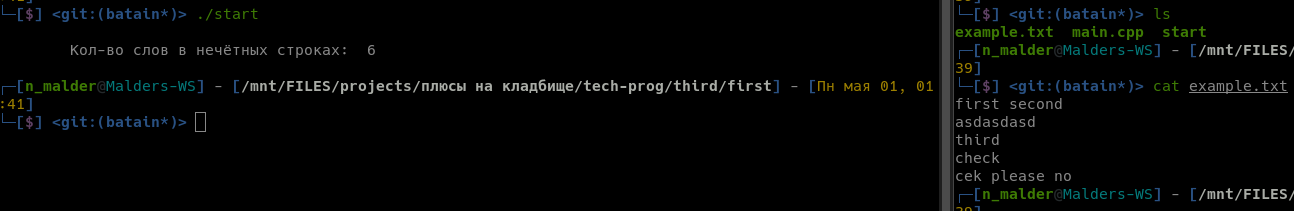
\includegraphics[width=1\textwidth]{1.png}
\newpage
\section{Задание №2} 
\subsection{Условие:}
Даны 3 комплексных числа. Посчитать бех использования библиотеки copmplex x = $\frac{a + b^3 + c}{a - b^2 - c}$
\subsection{Код:}
\scriptsize
\begin{verbatim}
#include <iostream>
using namespace std;
struct Complex { float Im; float Re; };
Complex Plus(Complex first, Complex second) {
    Complex summa;
    summa.Im = first.Im + second.Im;
    summa.Re = first.Re + second.Re;
    return summa;
}
Complex Minus(Complex first, Complex second) {
    Complex difference;
    difference.Im = first.Im - second.Im;
    difference.Re = first.Re - second.Re;
    return difference;
}
Complex Multiply(Complex first, Complex second) {
    Complex piece;
    piece.Re = first.Re * second.Re - first.Im * second.Im;
    piece.Im = first.Re * second.Im + second.Re * first.Im;
    return piece;
}
Complex Share(Complex first, Complex second) {
    Complex division;
    division.Re = (first.Re * second.Re + first.Im * second.Im) / (pow(second.Re, 2) + pow(second.Im, 2));
    division.Im = (second.Re * first.Im - first.Re * second.Im) / (pow(second.Re, 2) + pow(second.Im, 2));
    return division;
}
int main() {
    Complex x, num, den, a, b, c, buffer;
    cout << "Последовательно введите действительную и мнимую часть для\na: ";
    cin >> a.Im >> a.Re;
    cout << "b: "; cin >> b.Im >> b.Re;
    cout << "c: "; cin >> c.Im >> c.Re;
    buffer = Multiply(b, b);
    num = Plus(Plus(a, c), Multiply(buffer, b));
    den = Minus(Minus(a, buffer), c);
    x = Share(num, den);
    cout << "\nX.Re: " << x.Re << "\nX.Im:  " << x.Im << endl;
    return 0;
}\end{verbatim}\normalsize
\subsection{Результат:}
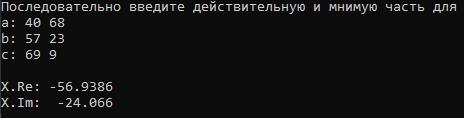
\includegraphics[width=1\textwidth]{2.png}
\newpage
\section{Задание №3} 
\subsection{Условие:}
Для заданных матриц комплексных чисел А(n×n) и B(n×n) найти C = (A^2 + B^2)^T.

Вычислить C^{-1}
\subsection{Код:}
\scriptsize
\begin{verbatim}
#include <iostream>
#include <fstream>
#include <cmath>
#include <complex>
#include <string>
using namespace std;
complex<int> Determ(complex<int>** matr, int n) {
    complex<int> det;
    if (n == 1) det = matr[n - 1][n - 1];
    if (n == 2)
        det = matr[0][0] * matr[1][1] - matr[0][1] * matr[1][0];
    if (n == 3) {
        det = matr[0][0] * matr[1][1] * matr[2][2] + matr[0][1] * matr[1][2] * matr[2][0] + matr[1][0] * matr[2][1] * matr[0][2];
        det -= matr[2][0] * matr[1][1] * matr[0][2] - matr[1][0] * matr[0][1] * matr[2][2] - matr[2][1] * matr[1][2] * matr[0][0];
    }
    return det;
}
int main() {
    ifstream size_matrix("matrix_A.txt"), matr_A("matrix_A.txt"), matr_B("matrix_B.txt");
    if (size_matrix.is_open() && matr_A.is_open() && matr_B.is_open()) {
        int n = 0, buf;
        string number;
        char symbol;
        while (symbol != '\n') {
            size_matrix >> number; n++;
            size_matrix.get(symbol);
        }
        n /= 2;
        size_matrix.close();
        complex<int>** A = new complex<int>*[n], ** B = new complex<int>*[n], ** C_T = new complex<int>*[n], ** C = new complex<int>*[n];
        for (int i = 0; i < n; i++) {
            A[i] = new complex<int>[n];
            B[i] = new complex<int>[n];
            C_T[i] = new complex<int>[n];
            C[i] = new complex<int>[n];
            for (int j = 0; j < n; j++) {
                matr_A >> buf; A[i][j].real(buf);
                matr_A >> buf; A[i][j].imag(buf);
                matr_B >> buf; B[i][j].real(buf);
                matr_B >> buf; B[i][j].imag(buf);
            }
        }
        matr_A.close();
        matr_B.close();
        cout << "A:\n";
        for (int i = 0; i < n; i++) {
            for (int j = 0; j < n; j++) cout << A[i][j] << " ";
            cout << endl;
        }
        cout << "\nB:\n";
        for (int i = 0; i < n; i++) {
            for (int j = 0; j < n; j++) cout << B[i][j] << " ";
            cout << endl;
        }
        cout << "\nC:\n";
        for (int i = 0; i < n; i++)
            for (int j = 0; j < n; j++)
                C_T[j][i] = A[i][j] * A[i][j] + B[i][j] * B[i][j];
        for (int i = 0; i < n; i++) {
            for (int j = 0; j < n; j++) cout << C_T[i][j] << " ";
            cout << endl;
        }
        cout << "\nC^-1:\n";
        complex<int> det = Determ(C_T, n);
        for (int i = 0; i < n; i++) {
            for (int j = 0; j < n; j++) {
                C[i][j] = C_T[j][i] / det;
                cout << C[i][j] << " ";
            }
            cout << endl;
        }
        for (int i = 0; i < n; i++) {
            delete[]A[i]; delete[]B[i];
            delete[]C_T[i]; delete[]C[i];
        }
        delete[]A; delete[]B;
        delete[]C_T; delete[]C;
    }
    return 0;
}\end{verbatim}\normalsize
\subsection{Результат:}
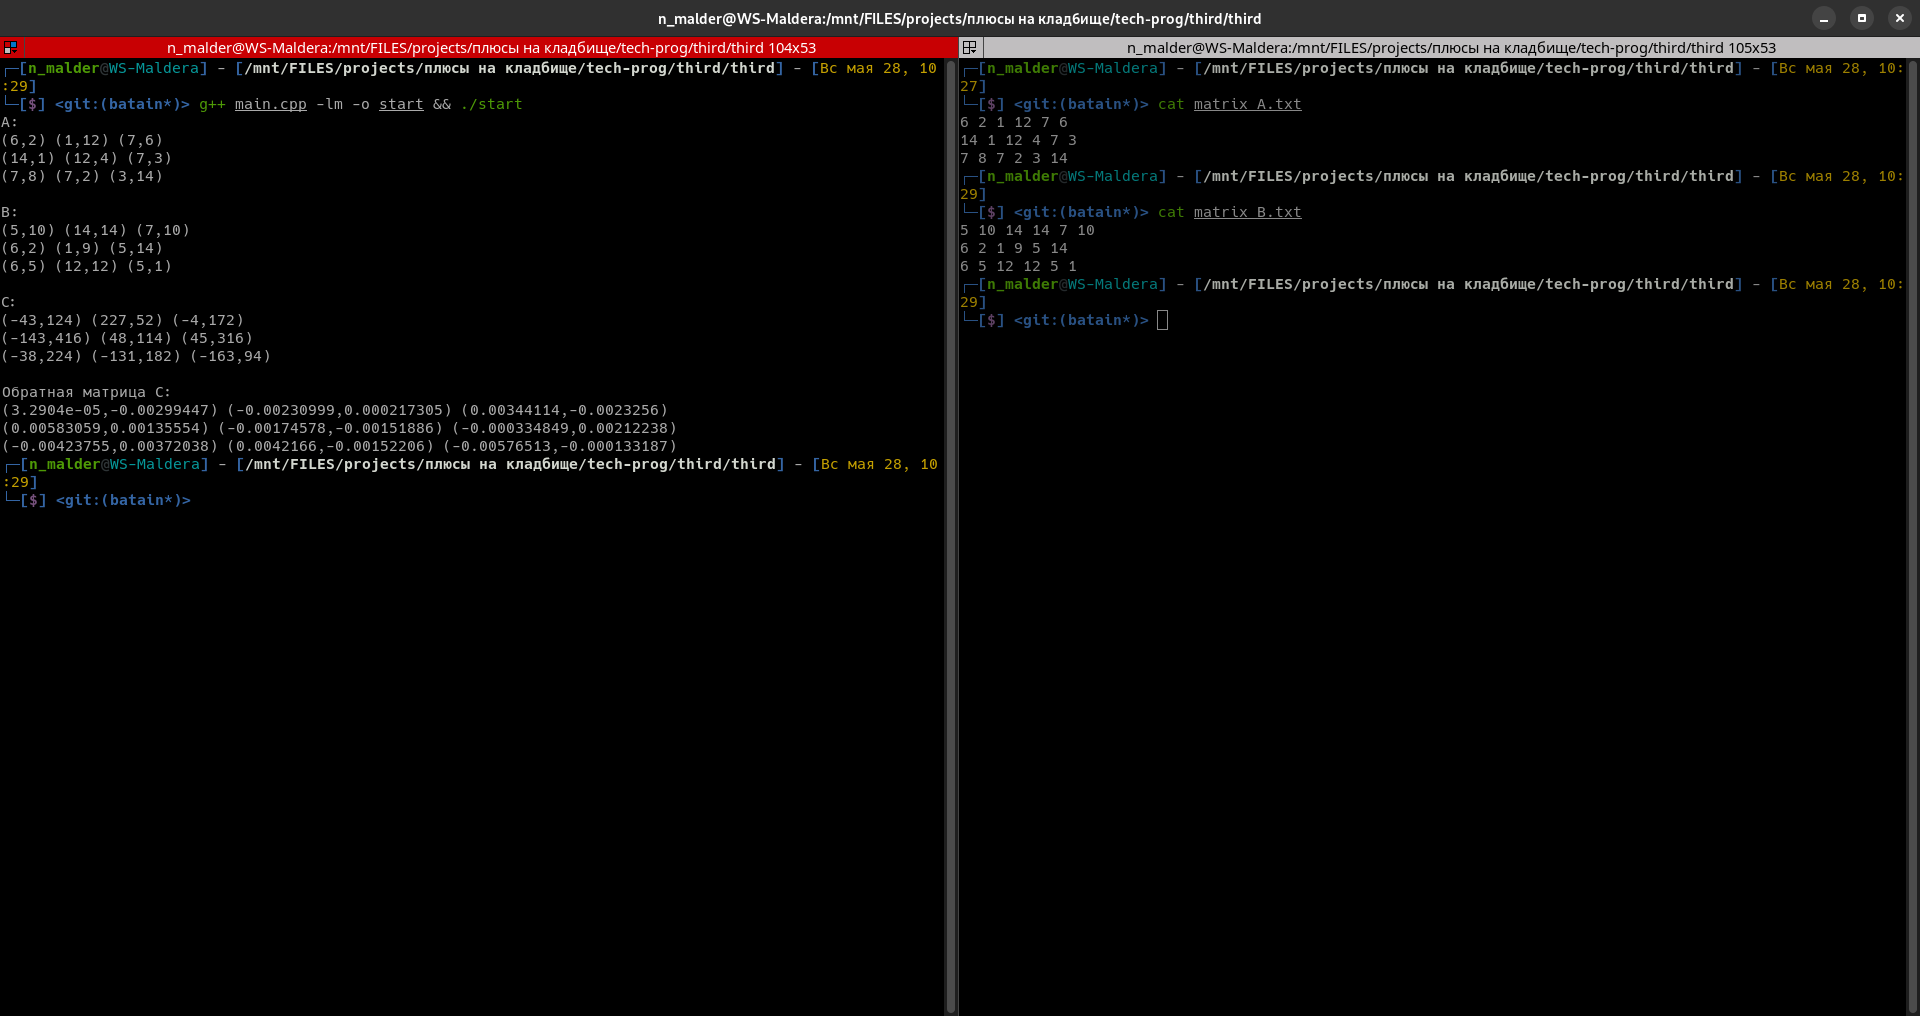
\includegraphics[width=1\textwidth]{3.png}
\subsection{Проверка через мат пакеты:}
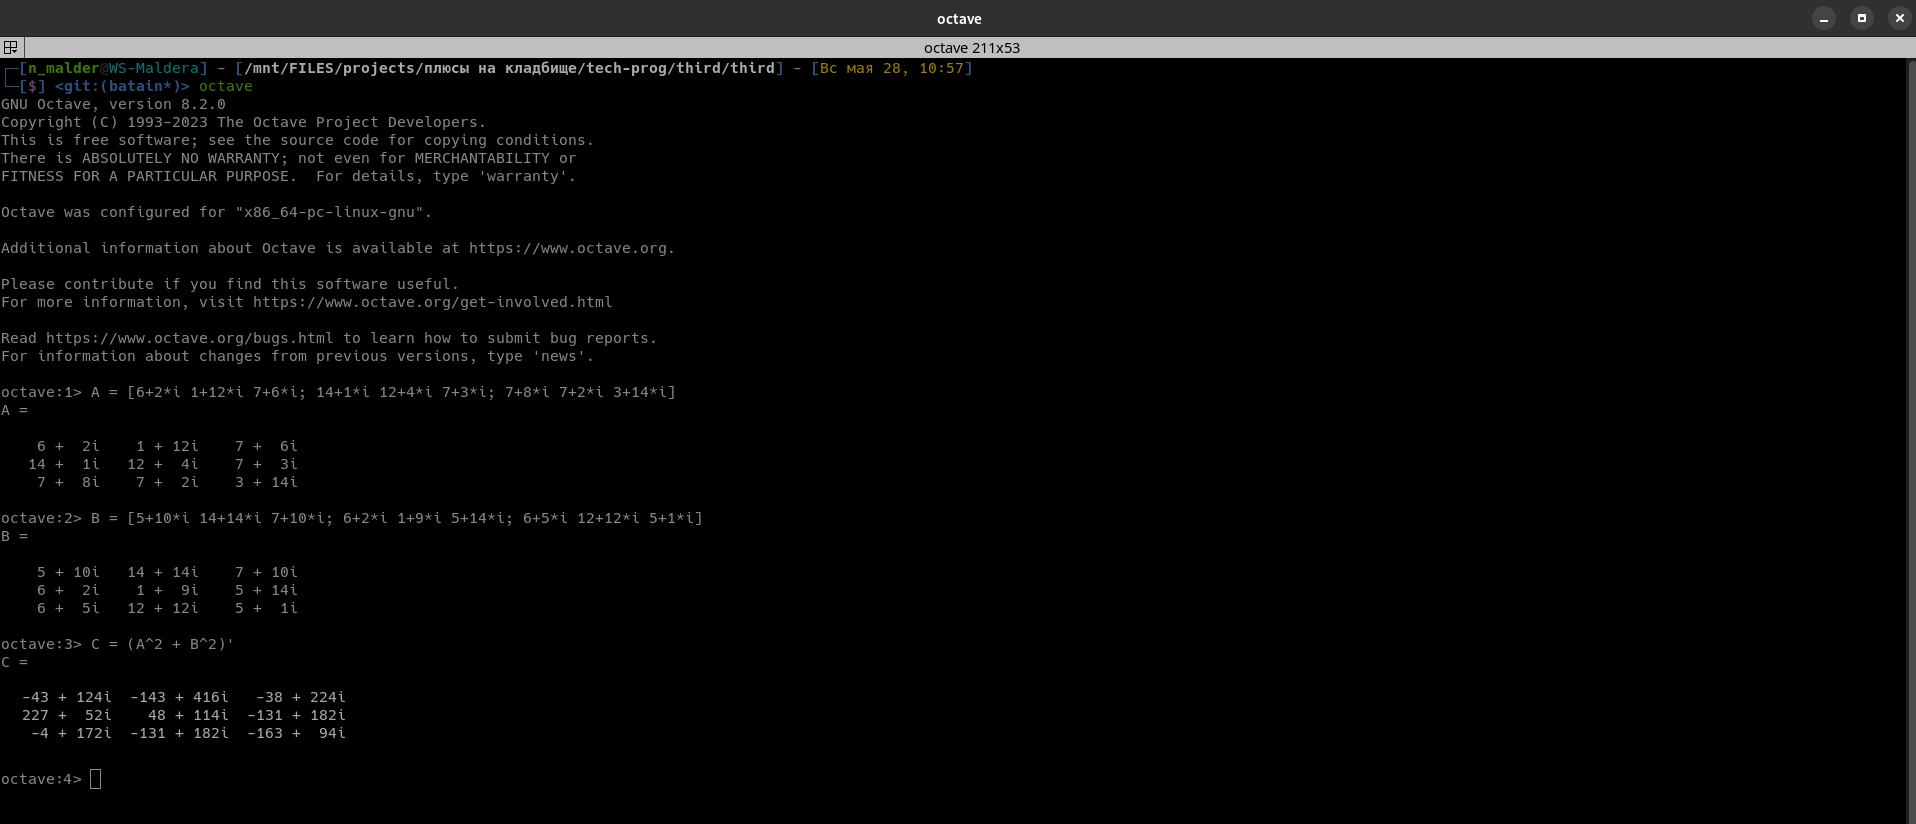
\includegraphics[width=1\textwidth]{check.png}
\end{document}